\chapter{Resultados}

Este capítulo apresenta os resultados obtidos nos experimentos feitos para validação das técnicas utilizadas neste trabalho, bem como o resultado final da aplicação.

É importante notar que apesar da limitação dos experimentos feitos para o rastreamento de pontos do rosto e para a estimação tridimensional foi possível obter dados suficientes para uma análise de precisão das técnicas.

\section{Calibração das Câmeras}

A Tabela \ref{tab:params_intrisecos} mostra os parâmetros intrínsecos das câmeras utilizadas obtidos utilizando a ferramenta \textit{Camera Calibration Toolbox for Matlab}.

\begin{table}[!htb]
\centering
\begin{tabular}{|c|c|c|}
\hline
Parâmetros intrínsecos & Câmera 1 (pixel) & Câmera 2 (pixel)\\ \hline
$f_c(1)$ & $854 \pm 4$ &  $834 \pm 6$ \\ \hline
$f_c(2)$ & $858 \pm 4$ & $836 \pm 6$ \\ \hline
$cc(1)$ & $298 \pm 6$ & $300 \pm 7$ \\ \hline
$cc(2)$ & $232 \pm 6$ & $217 \pm 7$ \\ \hline
$alpha_c$ & 0 & 0 \\ \hline
\end{tabular}

\caption{Parâmetros intrínsecos da câmera medidos em pixeis.}
\label{tab:params_intrisecos}
\end{table}

Como pode ser observado os valores de $f_c(1)$ e $f_c(2)$, referentes a distância focal medida em pixeis horizontais e verticais, são bem próximos para ambas as câmeras. Com isso pode-se assumir que a câmera possui um pixel quadrado e assim tem uma distância focal $f = (f_c(1) + f_c(2))/2$, sendo $f$ o valor em pixeis.

As câmeras utilizadas neste trabalho são do mesmo modelo e seu foco é ajustável. O foco das câmeras foi ajustado para ficar parecido, a partir de uma avaliação visual apenas. Todos estes fatores explicam os resultado similares obtidos para as duas câmeras.

A partir destes dados é possível estimar a profundidade de um ponto alvo utilizando a Equação \ref{eq:3d_Zequation} e assim estimar o valor de $X$ em centímetros, pelas Equações \ref{eq:3d_realX1} e \ref{eq:3d_realX1}, assim como estimar o valor de $Y$ em centímetros, pelas Equações \ref{eq:3d_realY1} e \ref{eq:3d_realY2}.

\section{Rastreamento de Pontos da Face}

Os experimentos realizados nesta seção foram feitos com o objetivo de avaliar a precisão da detecção de pontos da face utilizando a SDK \textit{CSIRO Face Analysis}, bem como justificar o uso de técnicas de estimação tridimensional e filtragem digital.

Duas poses foram avaliadas, a Pose Neutra e a Pose Sorrindo, com isso a razão de distância avaliada foi a do \textbf{comprimento dos lábios}, já que é essa razão que varia entre as poses e que consequentemente, após a filtragem, se torna um dos pesos aplicados ao modelo final.

Para ambas câmeras 1 e 2 foi obtida a média e o desvio padrão para essa razão de distância, em pixeis, a partir de vários valores de profundidade. A média e o desvio padrão foram calculados a partir do valores medidos em trinta imagens de uma face imóvel capturadas sucessivamente com intervalos de tempo menores que um segundo.

A Tabela \ref{tab:exp-px-variando-dist-cam1} exibe os valores obtidos através da câmera 1. Enquanto a Figura \ref{fig:graf-cam1-dsv-dist} mostra um gráfico da variação do desvio padrão do comprimento dos lábios, para a Pose Neutra e a para Sorrindo, em relação a distância entre a câmera 1 e o alvo.


\begin{table}[!htb]
\centering
\begin{tabular}{|*{6}{>{\centering\arraybackslash}p{.16\linewidth}|}}
\cline{2-5}
	\multicolumn{1}{c|}{} & \multicolumn{2}{c|}{Câmera 1 - Pose Neutra (pixel)} & \multicolumn{2}{c|}{Câmera 1 - Pose Sorrindo (pixel)} \\ \hline
    \begin{tabular}{@{}c@{}}Distância da \\ câmera (cm)\end{tabular} & Média &  Desvio padrão & Média &  Desvio padrão \\ \hline
40 & 93.4096 & 0.5575 & 92.1488 & 1.3473 \\ \hline
45 & 83.7242 & 0.6406 & 84.694  & 0.8848 \\ \hline
50 & 75.6548 & 0.7163 & 78.1044 & 1.0881 \\ \hline
55 & 67.9294 & 0.6772 & 69.1071 & 0.9671 \\ \hline
60 & 65.1105 & 0.3884 & 65.8582 & 0.8114 \\ \hline
65 & 58.8054 & 0.3392 & 59.7229 & 0.5219 \\ \hline
70 & 54.7137 & 0.5925 & 55.7597 & 0.6367 \\ \hline
75 & 53.4555 & 0.4781 & 53.7684 & 0.6277 \\ \hline
80 & 49.1185 & 0.3156 & 49.7219 & 0.2373 \\ \hline
\end{tabular}
\caption{Comprimento horizontal dos lábios medido em pixeis a partir de imagens capturadas do rosto alvo pela câmera 1 em distâncias variáveis.}
\label{tab:exp-px-variando-dist-cam1}
\end{table}

\begin{figure}[!htb]
\centering
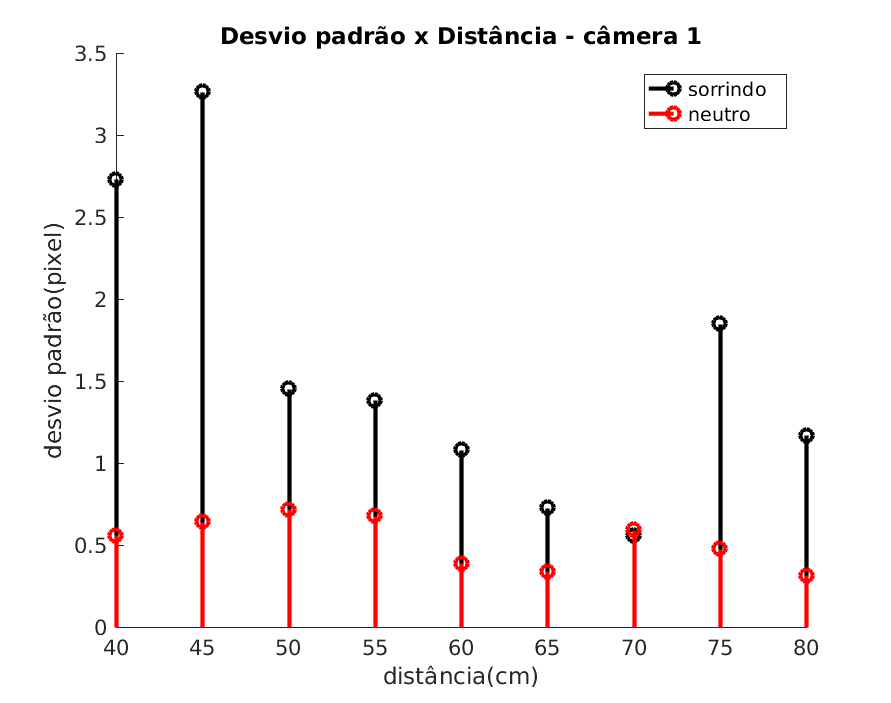
\includegraphics[width=0.8\textwidth]{figs/thumbnail_cameraEsquerda.jpg} 
\caption{Gráfico da variação do desvio padrão, em pixeis, em relação a distância, em centímetros, de pontos rastreados nas imagens capturadas pela câmera 1.}
\label{fig:graf-cam1-dsv-dist}
\end{figure}

A Tabela \ref{tab:exp-px-variando-dist-cam2} exibe os valores obtidos através da câmera 2. Enquanto a Figura \ref{fig:graf-cam2-dsv-dist} mostra um gráfico da variação do desvio padrão do comprimento dos lábios, para a Pose Neutra e a para Sorrindo, em relação a distância entre a câmera 2 e o alvo.

\begin{table}[!htb]
\centering
\begin{tabular}{|*{6}{>{\centering\arraybackslash}p{.16\linewidth}|}}
\cline{2-5}
	\multicolumn{1}{c|}{} & \multicolumn{2}{c|}{Câmera 2 - Pose Neutra (pixel)} & \multicolumn{2}{c|}{Câmera 2 - Pose Sorrindo (pixel)} \\ \hline
    \begin{tabular}{@{}c@{}}Distância da \\ câmera (cm)\end{tabular} & Média &  Desvio padrão & Média &  Desvio padrão \\ \hline
40 & 92.1488 & 1.3473 & 119.6076 & 2.2723 \\ \hline
45 & 84.694  & 0.8848 & 106.7452 & 2.23   \\ \hline
50 & 78.1044 & 1.0881 & 108.4763 & 1.2881 \\ \hline
55 & 69.1071 & 0.9671 & 94.7001  & 1.2003 \\ \hline
60 & 65.8582 & 0.8114 & 87.5216  & 0.5491 \\ \hline
65 & 59.7229 & 0.5219 & 82.719   & 0.9558 \\ \hline
70 & 55.7597 & 0.6367 & 75.3994  & 0.4099 \\ \hline
75 & 53.7684 & 0.6277 & 67.9172  & 1.0836 \\ \hline
80 & 49.7219 & 0.2373 & 68.2629  & 1.0946 \\ \hline
\end{tabular}
\caption{Comprimento horizontal dos lábios medido em pixeis a partir de imagens capturadas do rosto alvo pela câmera 2 em distâncias variáveis.}
\label{tab:exp-px-variando-dist-cam2}
\end{table}

\begin{figure}[!htb]
\centering
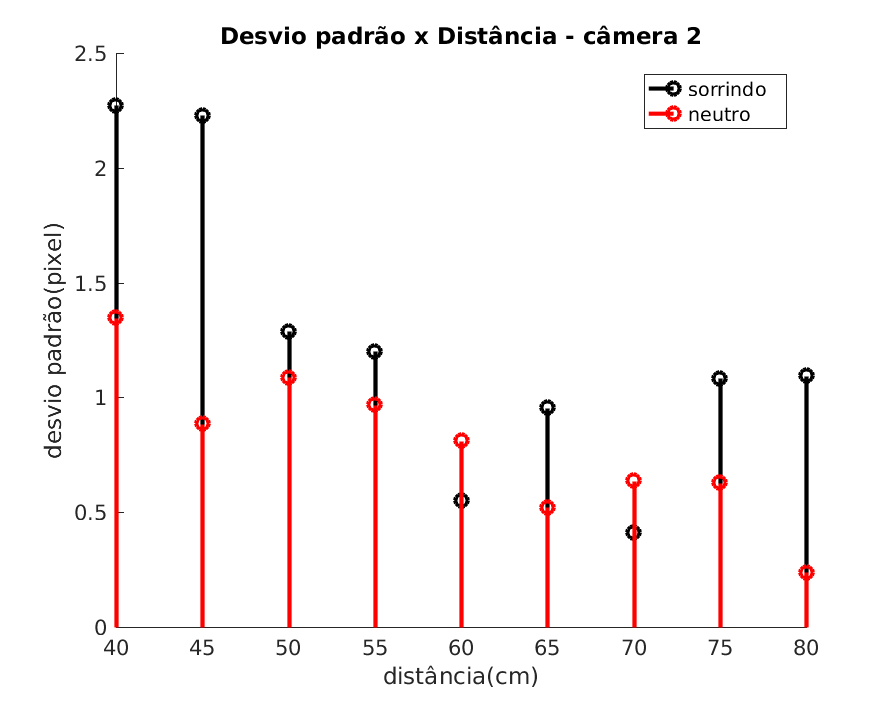
\includegraphics[width=0.8\textwidth]{figs/thumbnail_cameraDireita.jpg} 
\caption{Gráfico da variação do desvio padrão, em pixeis, em relação a distância, em centímetros, de pontos rastreados nas imagens capturadas pela câmera 2.}
\label{fig:graf-cam2-dsv-dist}
\end{figure}

Os gráficos exibidos na Figura \ref{fig:graf-cam1-dsv-dist} e na Figura \ref{fig:graf-cam2-dsv-dist} mostram que existe uma instabilidade no rastreamento de pontos da face, que apesar de pequena pode afetar o modelo final. Essa variação dos pontos acontecem em altas frequências, visto que as imagens foram capturadas sucessivamente em pequenos intervalos de tempo, assim essa instabilidade pode ser tratada com a utilização de filtragem digital. 

Outro comportamento exibido pelos gráficos é o de que o desvio padrão é quase sempre maior quando a razão de distância é medida na Pose Sorrindo do que quando ela é medida na Pose Neutra, ou seja, o rastreamento geralmente é mais estável quando feito em uma face sem expressões.

Como observado o desvio padrão em geral diminui com o aumento da distância, porém esse acontecimento pode ser atribuído ao fato de que, como a razão de distância esta avaliada em pixeis, quanto maior a distância menor o valor da razão de distância.

Observando as tabelas é possível reparar na diminuição drástica da média a medida que o valor de profundidade aumenta, de forma que o valor obtido do comprimento dos lábios a uma distância de 80cm é quase a metade do valor a 40cm. 

Essa mudança brusca impossibilita uma boa calibração para as razões de distância, visto que a razão de distância, e consequentemente o modelo final, pode mudar com uma variação de profundidade, mesmo se o alvo estiver na mesma pose. Para isso é usada a estimação tridimensional, com ela é possível manter uma mesma razão de distância, caso a pose seja a mesma, não importa a profundidade, não alterando assim o modelo final.

\section{Estimação do Tridimensional}

O objetivo dos experimentos nessa seção é avaliar a precisão da técnica de estimação tridimensional. Deve-se notar que uma precisão na estimação do $X$ e do $Y$ no sistema de coordenadas do mundo só é possível caso haja precisão na estimação do $Z$, como pode ser observado nas Equações \ref{eq:3d_realX1}, \ref{eq:3d_realX2}, \ref{eq:3d_realY1} e \ref{eq:3d_realY2}.

Como nos experimentos da seção anterior, em que foi avaliada a precisão do rastreamento de pontos da face, a razão de distância analisada foi a referente ao comprimento dos lábios. Foram utilizadas as mesmas imagens, porém agora essa razão de distância foi estimada em centímetros, ou seja os pontos foram estimados no sistema de coordenadas do mundo.

A Tabela \ref{tab:exp-px-variando-dist-3d} exibe os valores estimados em centímetros. Enquanto a Figura \ref{fig:graf-3d-dsv-dist} e a Figura \ref{fig:graf-3d-media-dist} mostram um gráfico da variação do desvio padrão e da média, respectivamente, do comprimento dos lábios, para a Pose Neutra e a para Sorrindo, em relação a distância entre as câmeras e o alvo.


\begin{table}[!htb]
\centering
\begin{tabular}{|*{6}{>{\centering\arraybackslash}p{.16\linewidth}|}}
\cline{2-5}
	\multicolumn{1}{c|}{} & \multicolumn{2}{c|}{Pose Neutra (cm)} & \multicolumn{2}{c|}{ Pose Sorrindo (cm)} \\ \hline
    \begin{tabular}{@{}c@{}}Distância da \\ câmera (cm)\end{tabular} & Média &  Desvio padrão & Média &  Desvio padrão \\ \hline
40 & 5.2755 & 0.1155 & 6.8652 & 0.2549 \\ \hline
45 & 5.5857 & 0.0991 & 6.8311 & 0.1564 \\ \hline
50 & 5.4356 & 0.0959 & 7.3474 & 0.116  \\ \hline
55 & 5.3663 & 0.1135 & 7.3599 & 0.1574 \\ \hline
60 & 5.5722 & 0.1144 & 7.4396 & 0.1107 \\ \hline
65 & 5.4381 & 0.0932 & 7.4996 & 0.1433 \\ \hline
70 & 5.8243 & 0.0879 & 7.7648 & 0.1024 \\ \hline
75 & 5.7759 & 0.1494 & 7.1711 & 0.2339 \\ \hline
80 & 5.5645 & 0.0716 & 7.7803 & 0.1659 \\ \hline
\end{tabular}
\caption{Comprimento horizontal dos lábios medido em centímetros a partir de imagens capturadas do rosto alvo em distâncias variáveis.}
\label{tab:exp-px-variando-dist-3d}
\end{table}

\begin{figure}[!htpb]
\centering
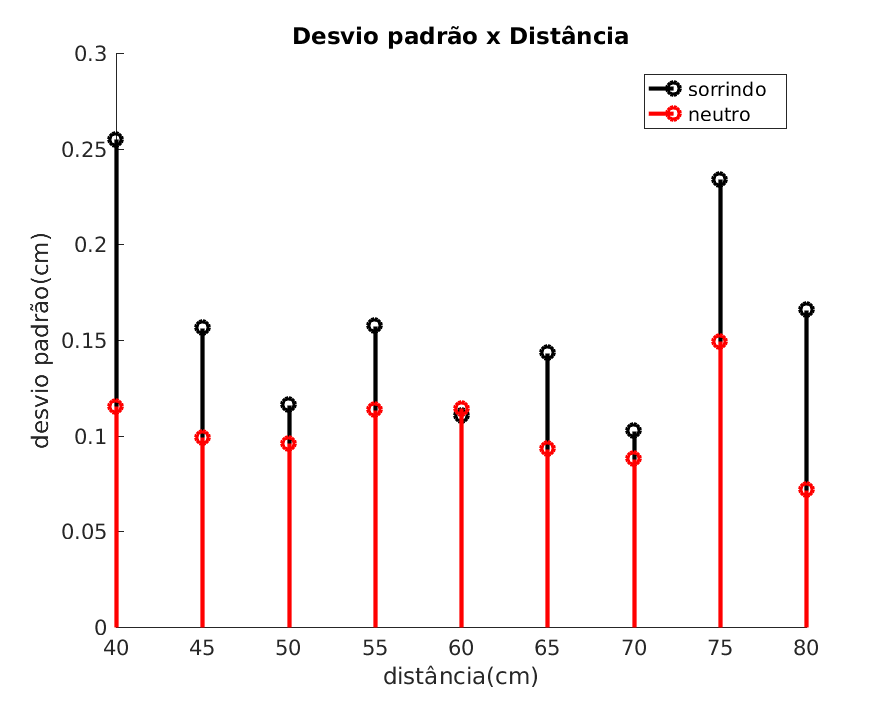
\includegraphics[width=0.8\textwidth]{figs/thumbnail_distanciaCorrigida.jpg} 
\caption{Gráfico da variação do desvio padrão, em centímetros, em relação a distância, em centímetros, de pontos estimados no sistema de coordenadas do mundo.}
\label{fig:graf-3d-dsv-dist}
\end{figure}

O gráfico exibido na Figura \ref{fig:graf-3d-dsv-dist} mostra o desvio padrão do valor em centímetros da razão de distância, ele pode ser diretamente relacionado com a instabilidade do rastreamento de pontos. Essa instabilidade é exibida na Figura \ref{fig:graf-cam1-dsv-dist} e na Figura \ref{fig:graf-cam2-dsv-dist}. 

\begin{figure}[!htpb]
\centering
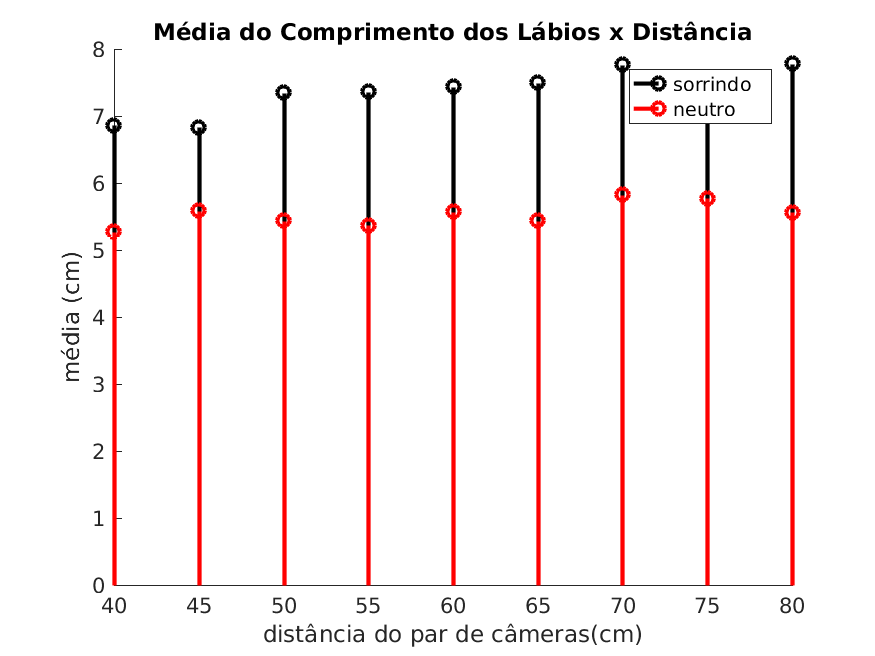
\includegraphics[width=0.8\textwidth]{figs/media3d.png} 
\caption{Gráfico da variação média, em centímetros, em relação a distância, em centímetros, de pontos estimados no sistema de coordenadas do mundo.}
\label{fig:graf-3d-media-dist}
\end{figure}

A precisão da estimação tridimensional pode ser verificada ao se avaliar a variação da média em relação a distância. Esses dados são exibidos na Figura \ref{fig:graf-3d-media-dist}, nota-se que a média se mantém suficientemente constante, principalmente nos intervalos entre 50cm e 65cm. Com isso pode-se concluir que mesmo que aconteça uma variação da distância do alvo em relação as câmeras, a razão de distância se manterá estável, garantindo estabilidade para o modelo final.

\section{Filtros}

Neste experimentos foram gerados gráficos de sequências para os pesos de mistura de 3 das poses utilizadas. Cada gráfico mostra medidas de pesos de mistura para uma das poses, com um curva para os valor não-filtrado e curvas para alguns dos filtros projetados.  As sequências foram obtidas em um vídeo gravado com o objetivo de movimentar especificamente a pose sendo testada. Os gráficos foram gerados selecionando-se parte das sequências gravadas.

A Figuras \ref{fig:filter-left-eye}, \ref{fig:filter-open-mouth} e \ref{fig:filter-smile} demonstram a atuação dos filtros sobre a variação do peso de mistura para as poses Olho Esquerdo, Boca Aberta e Sorriso.

\begin{figure}[!htb]
\centering
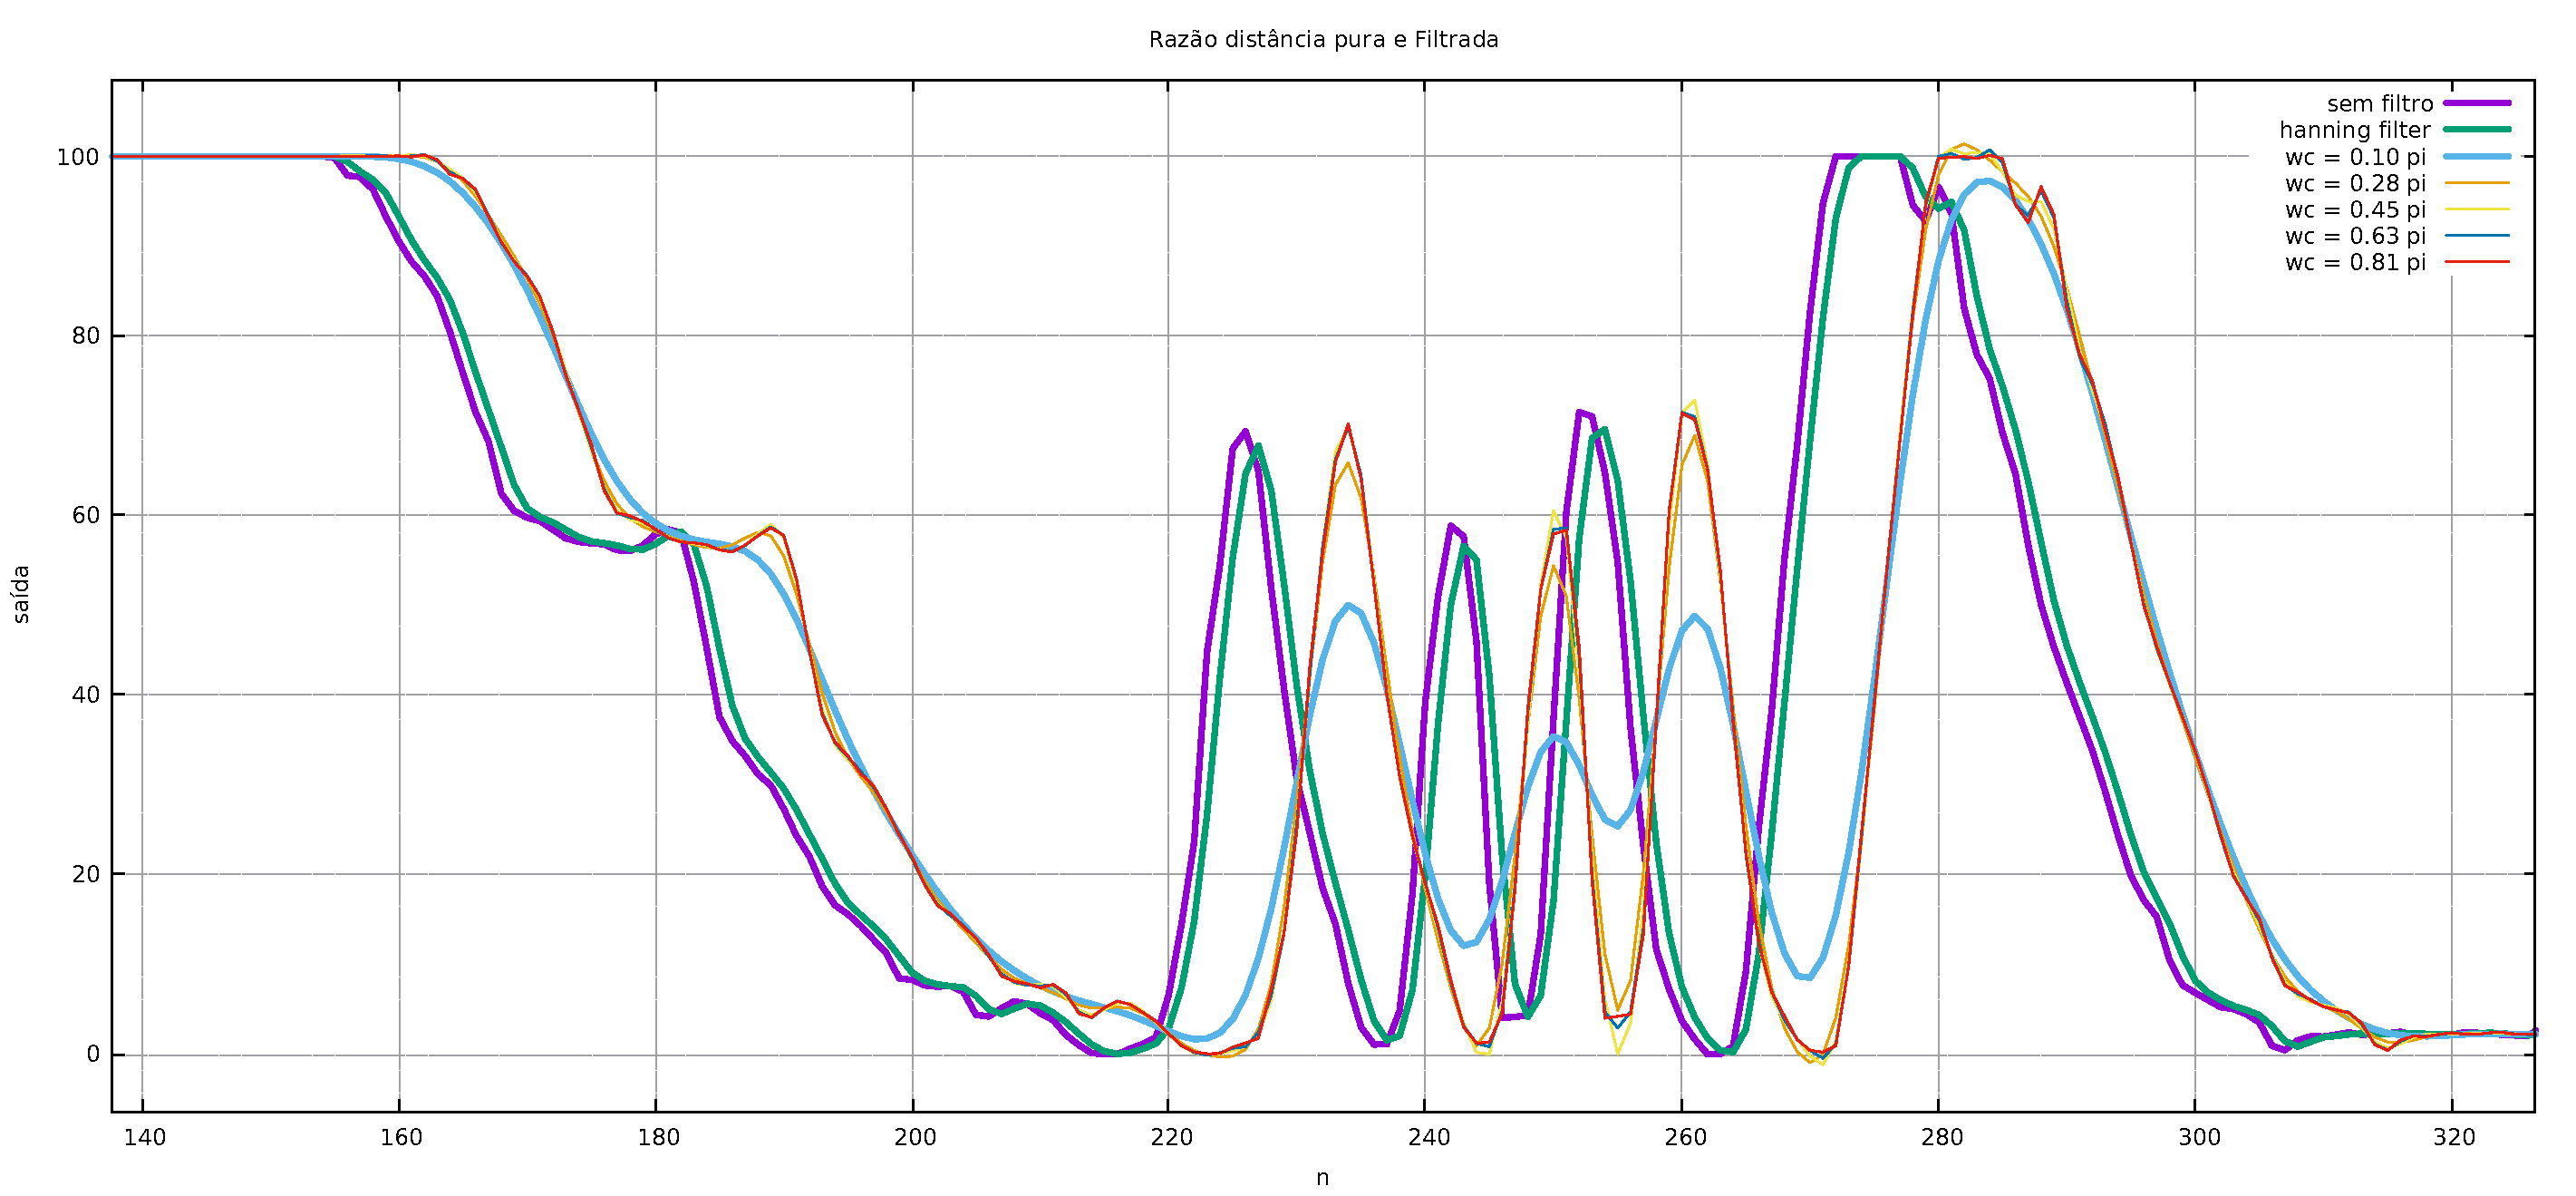
\includegraphics[width=1.0\textwidth]{figs/filter-result-open-mouth.pdf} 
\caption{Peso de mistura para a Pose Olho Esquerdo}
\label{fig:filter-left-eye}
\end{figure}

\begin{figure}[!htb]
\centering
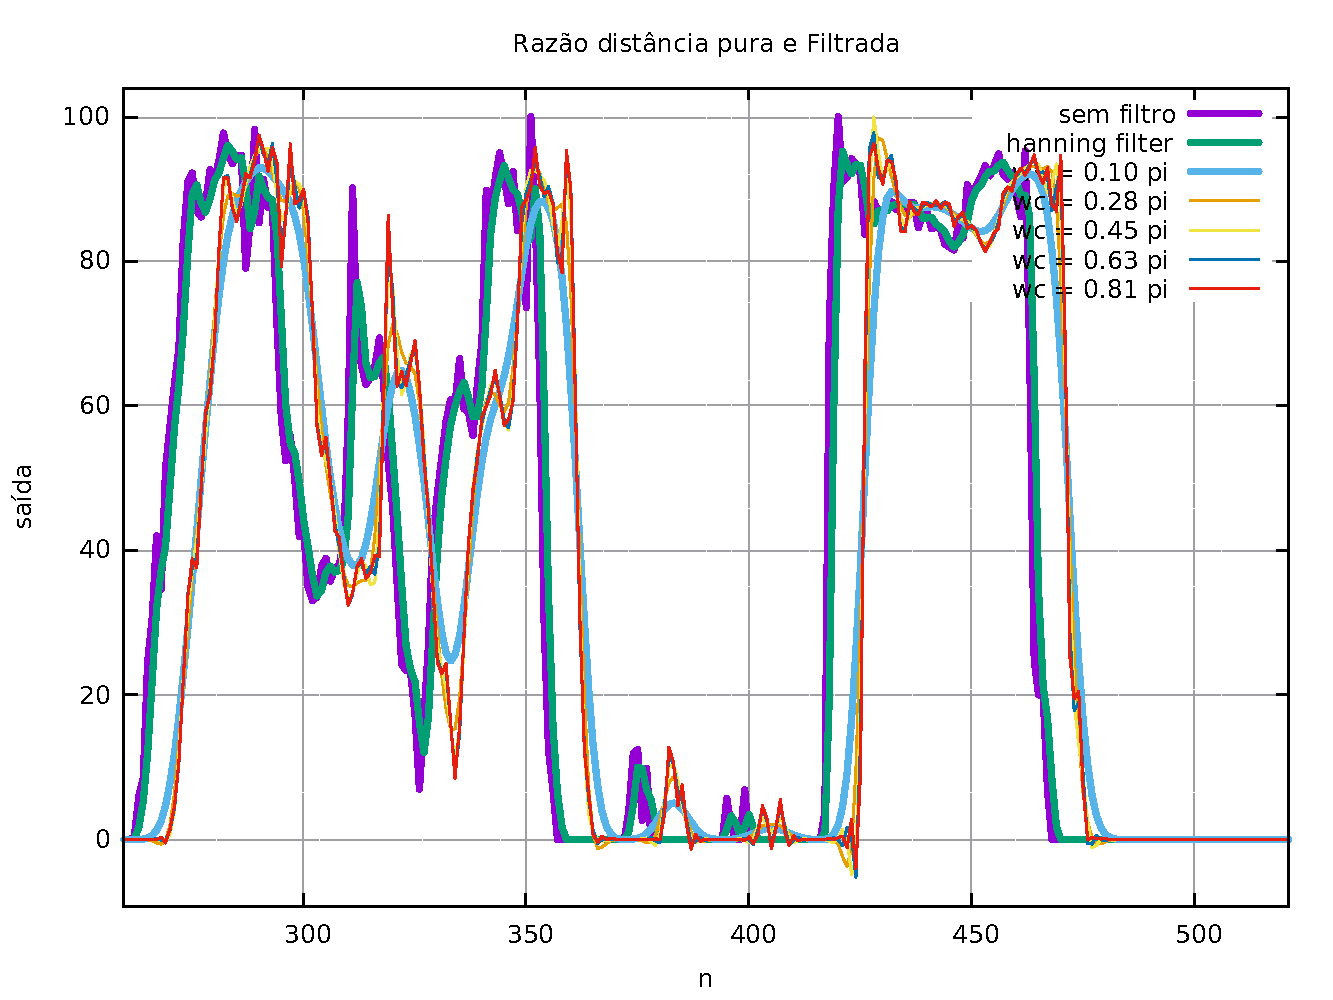
\includegraphics[width=0.8\textwidth]{figs/filter-result-left-eye.pdf} 
\caption{Peso de mistura para a Pose Boca Aberta}
\label{fig:filter-open-mouth}
\end{figure}

\begin{figure}[!htb]
\centering
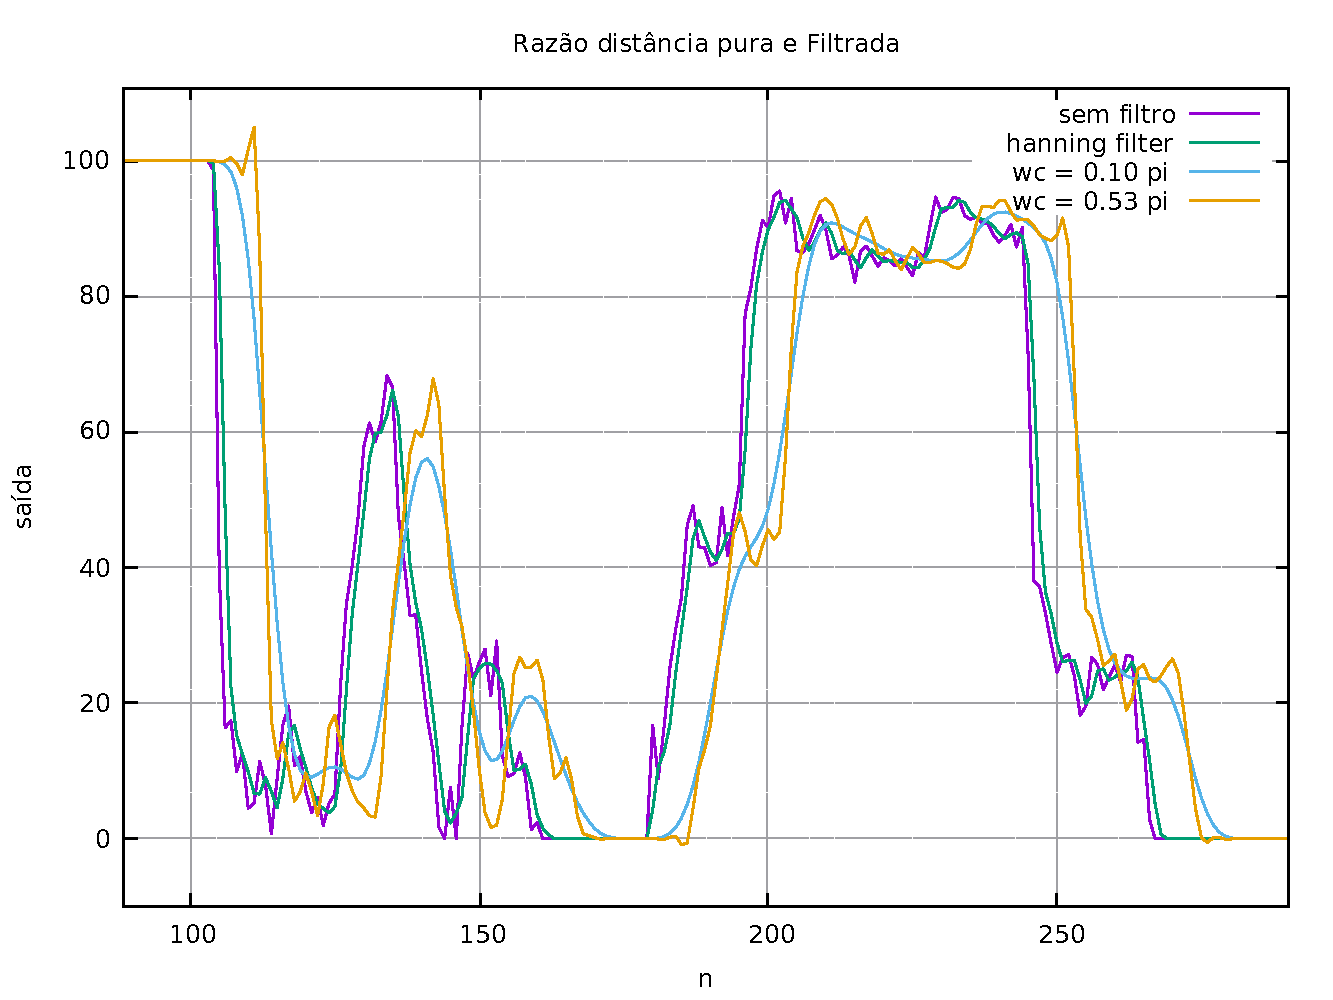
\includegraphics[width=0.8\textwidth]{figs/filter-result-smile-2.pdf} 
\caption{Peso de mistura para a Pose Sorriso}
\label{fig:filter-smile}
\end{figure}

Como visto nas Figuras \ref{fig:graf-cam1-dsv-dist} e \ref{fig:graf-cam2-dsv-dist} o rastreamento em si não é totalmente preciso nem quando o rosto está imóvel, logo em um vídeo longo onde ocorre movimentação e variação de luminosidade é esperado que o sinal sem filtragem seja mais ruidoso, como é mostrados no gráficos. 

A filtragem suaviza o sinal e consequentemente melhora a animação final. Vários tipos de filtro foram analisados e seus desempenhos foram variados.

Como pode ser observado os filtros projetados pela técnica de janela acabam atrasando atrasando o sinal e, apesar de eles serem eficientes em filtrar altas frequências, esses tipos de filtro acabam prejudicando a performance da animação em tempo real.

Por outro lado o filtro de hanning conseguiu seguir o sinal original e manter uma boa filtragem das altas frequências, isso acontece pois este tipo de filtro possui muito menos parâmetros que os outros projetados. Para este trabalho, onde um dos objetivos é a animação em tempo real, esse tipo filtro apresentou o melhor resultado.

\section{Mistura de Poses}

Neste experimento foi avaliada somente a técnica de mistura de poses, ou seja, foi renderizado um modelo final sem a influência do rastreamento de pontos da face. Para isso foram atribuídos manualmente os valores de peso.

Alguns exemplos de modelos finais de poses intermediárias renderizados com sucesso podem ser vistos na Figura \ref{fig:blend-shapes-inter-simple-shapes}.

\begin{figure}[!htb]
  \centering
  \begin{subfigure}[]{\label{fig:inter1}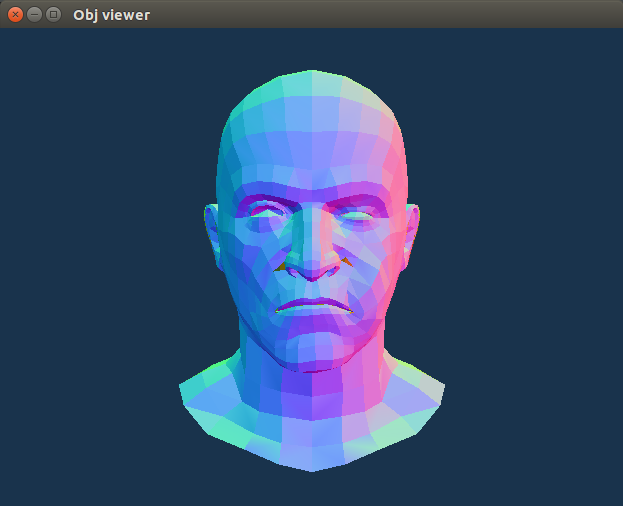
\includegraphics[width=0.4\textwidth]{./figs/TG_angry60_leftcheek75_lefteye55_closemouth35.png}}
  \end{subfigure}   
  \begin{subfigure}[]{\label{fig:inter2}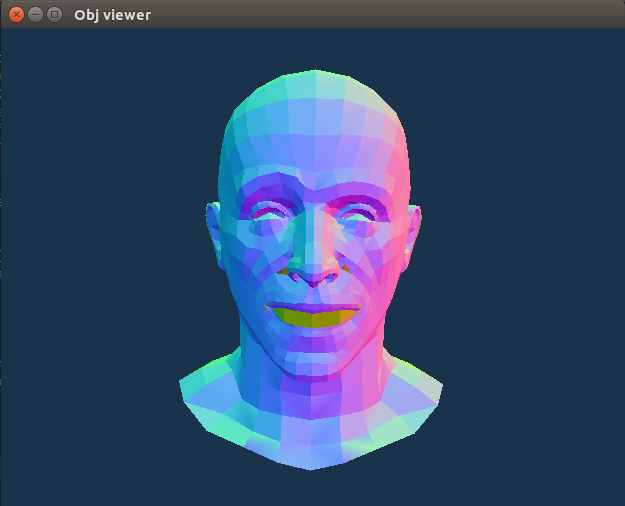
\includegraphics[width=0.4\textwidth]{./figs/TG_happy40_righteyebrow95_openmouth60.png}}
  \end{subfigure}
  
  \begin{subfigure}[]
  {\label{fig:inter3}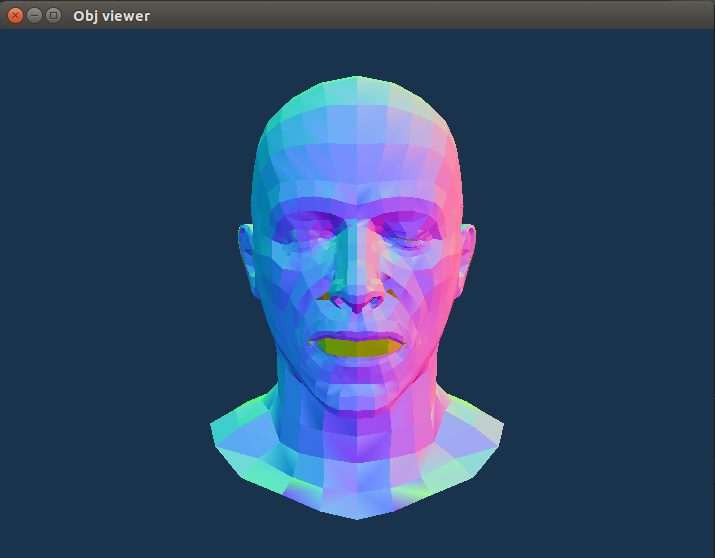
\includegraphics[width=0.4\textwidth]{./figs/TG_lefteye100_rigtheye100_openmouth60.png}}
  \end{subfigure} 
  \begin{subfigure}[]
  {\label{fig:inter4}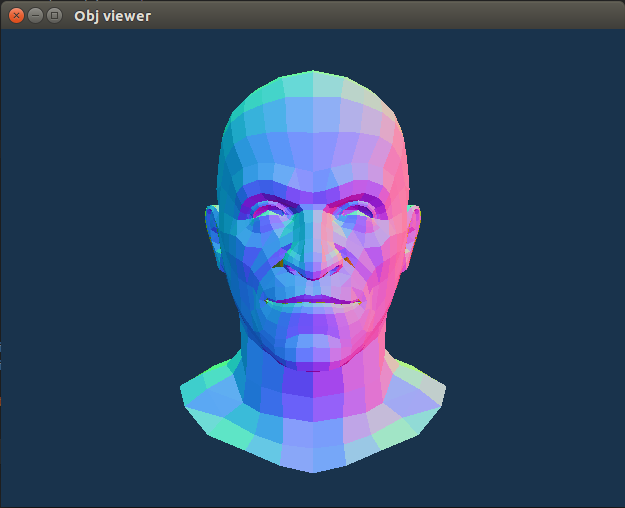
\includegraphics[width=0.4\textwidth]{./figs/TG_happy70_angry90.png}}
  \end{subfigure}
  
  \begin{subfigure}[]{\label{fig:inter5}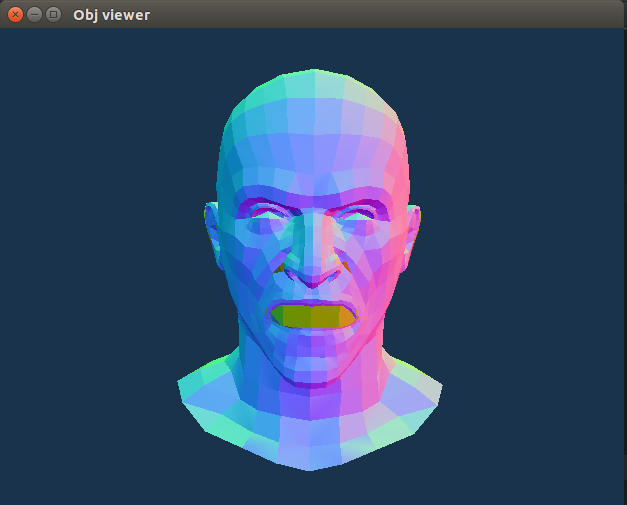
\includegraphics[width=0.4\textwidth]{./figs/TG_angry100_openmouth90.png}}
  \end{subfigure}
  \begin{subfigure}[]{\label{fig:inter6}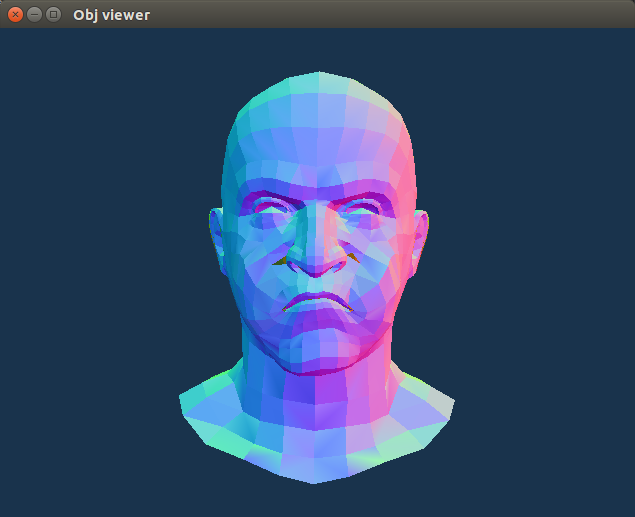
\includegraphics[width=0.4\textwidth]{./figs/TG_angry100_leftcheek100_rightcheek65_closemouth100.png}}
  \end{subfigure}

  \caption{Exemplo de misturas geradas configurando os parâmetros de mistura manualmente. Pesos da Figura \ref{fig:inter1}: Olho Esquerdo - 0.55, Boca Fechada - 0.35, Bochecha Esquerda - 0.75 e Bravo - 0.6. Pesos da Figura \ref{fig:inter2}: Sobrancelha Direita - 0.95, Boca Aberta - 0.6 e Sorrindo - 0.4. Pesos da Figura \ref{fig:inter3}: Olho Esquerdo - 1.0, Olho Direito - 1.0 e Boca Aberta - 0.6. Pesos da Figura \ref{fig:inter4}: Sorrindo - 0.7 e Bravo - 0.6. Pesos da Figura \ref{fig:inter5}: Boca Aberta - 1.0 e Bravo - 0.9. Pesos da Figura \ref{fig:inter6}: Boca Fechada - 1.0, Bochecha Esquerda - 1.0, Bochecha Direita - 0.65, e Bravo - 1.0.}

  \label{fig:blend-shapes-inter-simple-shapes}
\end{figure}

Como pode ser observado nos modelos finais exibidos a técnica de mistura de poses teve ótimos resultados. 

A indexação dos VBOs e a ordenação dos vetores foi constante, pois se não sendo este o caso seria possível observar algumas falhas óbvias no modelo, como alguns buracos aparecendo ou deformações irregulares se formando.

As significância de cada pose pré-definida no modelo final está bem relacionada com os pesos aplicados e essa relação pode ser claramente visualizada nas figuras, ou seja, ao aplicar a Equação \ref{eq:blendshapes} é possível criar, a partir de poucas poses pré-definidas, uma quantidade enorme de poses intermediárias significativamente diferentes.

Com esses resultados pode se concluir que caso ocorra uma boa estimação das razões de distância, a partir de um rastreamento de pontos, estimação tridimensional e filtragem, o modelo final correto será renderizado com sucesso.

\section{Sistema em Funcionamento}

A avaliação do sistema em funcionamento, similarmente ao que foi feito para a mistura de poses, é qualitativa. Quadros comparativos entre a imagem de entrada e o modelo final foram exibidos na \ref{fig:sist-func}, de forma a observar a qualidade da animação, avaliando o impacto do movimento dos pontos utilizados como referências para as razões de distância no modelo final. Para isso é necessária uma boa calibração dos valores de distância mínima e máxima para cada razão de distância. Esta avaliação é porém embasada nos resultados dos experimento obtidos para cada etapa.

O sistema em funcionamento pode ser observado na Figura \ref{fig:sist-func} em que o modelo final segue os movimentos do rosto alvo a partir das razões de distância consideradas.

\begin{figure}[!htb]
  \centering
  \begin{subfigure}[]{\label{fig:inter1}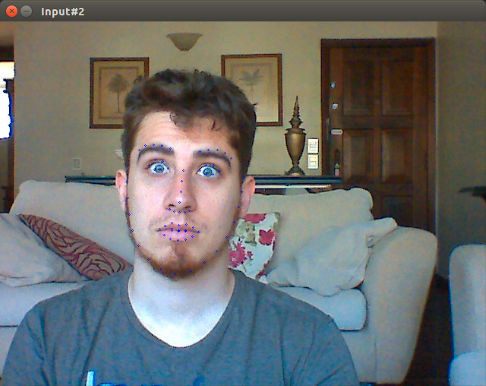
\includegraphics[width=0.35\textwidth]{./figs/TG-resultado-par-4-img-1.png}}
  \end{subfigure}   
  \begin{subfigure}[]{\label{fig:inter2}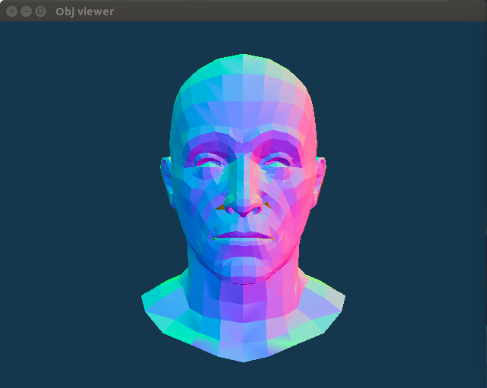
\includegraphics[width=0.35\textwidth]{./figs/TG-resultado-par-4-img-2.png}}
  \end{subfigure}
  
  \begin{subfigure}[]
  {\label{fig:inter3}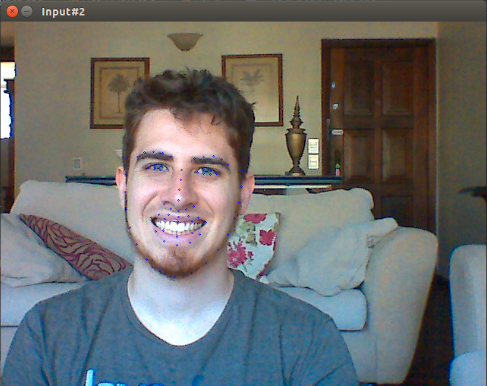
\includegraphics[width=0.35\textwidth]{./figs/TG-resultado-par-5-img-1.png}}
  \end{subfigure} 
  \begin{subfigure}[]
  {\label{fig:inter4}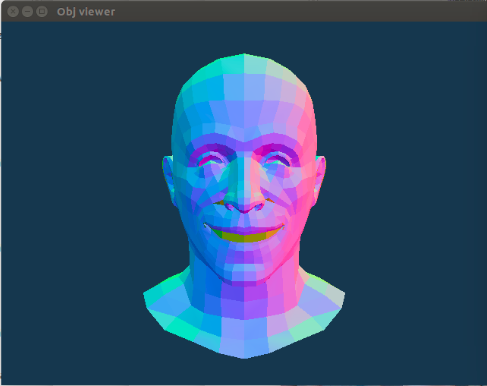
\includegraphics[width=0.35\textwidth]{./figs/TG-resultado-par-5-img-2.png}}
  \end{subfigure}

  \caption{Imagens que demonstram o sistema em funcionamento.}

  \label{fig:sist-func}
\end{figure}


